\documentclass{article}

% if you need to pass options to natbib, use, e.g.:
% \PassOptionsToPackage{numbers, compress}{natbib}
% before loading nips_2016
%
% to avoid loading the natbib package, add option nonatbib:
%\usepackage[nonatbib]{nips_2016}

%\usepackage{nips_2016}

% to compile a camera-ready version, add the [final] option, e.g.:
\usepackage[final]{nips_2016}

\usepackage[utf8]{inputenc} % allow utf-8 input
\usepackage[T1]{fontenc}    % use 8-bit T1 fonts
\usepackage{hyperref}       % hyperlinks
\usepackage{url}            % simple URL typesetting
\usepackage{booktabs}       % professional-quality tables
\usepackage{amsfonts}       % blackboard math symbols
\usepackage{nicefrac}       % compact symbols for 1/2, etc.
\usepackage{microtype}      % microtypography
\usepackage{graphicx}
\usepackage{makecell}
\usepackage{algorithm}% http://ctan.org/pkg/algorithms
\usepackage{algpseudocode}%
\usepackage{bm}
\usepackage{amsmath}
\usepackage{makecell}

\title{Optimizing Illumination for Overlapped Imaging}

% The \author macro works with any number of authors. There are two commands
% used to separate the names and addresses of multiple authors: \And and \AND.
%
% Using \And between authors leaves it to LaTeX to determine where to break the
% lines. Using \AND forces a line break at that point. So, if LaTeX puts 3 of 4
% authors names on the first line, and the last on the second line, try using
% \AND instead of \And before the third author name.

\author{%
  Amey A. Chaware\\
  Department of Electrical and Computer Engineering\\
  Duke University\\
  Durham, NC 27705 \\
  \texttt{amey.chaware@duke.edu} \\
  % examples of more authors
  % \And
  % Coauthor \\
  % Affiliation \\
  % Address \\
  % \texttt{email} \\
  % \AND
  % Coauthor \\
  % Affiliation \\
  % Address \\
  % \texttt{email} \\
  % \And
  % Coauthor \\
  % Affiliation \\
  % Address \\
  % \texttt{email} \\
  % \And
  % Coauthor \\
  % Affiliation \\
  % Address \\
  % \texttt{email} \\
}

\begin{document}
% \nipsfinalcopy is no longer used

\maketitle

\begin{abstract}
  
We present an imaging system that simultaneously captures multiple images and automatically classifies their contents to increase detection throughput. Our optical design consists of a set of multiple lenses that each image a unique field-of-view onto a single image sensor. The resulting ``overlapped" image exhibits reduced contrast, but includes measurements from across a proportionally larger viewing area. We then post-process this overlapped image with a deep convolutional neural network to classify the presence or absence of certain features of interest. Additionally, we explore the use of machine learning to jointly optimize the illumination for this task of classification in overlapped images. We demonstrate that it is possible to overlap multiple unique images onto a common sensor while still offering accurate classification and that this performance is improved by using optimized image capture process.

\end{abstract}

\section{Introduction}

One particular challenge with optical imaging systems, and microscopes in particular, is to simultaneously image a large area at high resolution (i.e., extend beyond megapixels and into gigapixels). For example, independent of the exact lens that is used, most standard microscopes are limited to capture just 50 megapixels per image~\cite{Zheng14}. At 1 micrometer resolution, imaging throughput drops to approximately 15 megapixels per image. This limit is not caused by electronics - computers are certainly capable of reading in more than 50 megapixels per snapshot. Instead, it is primarily caused by imperfections in large lenses (i.e., lens aberrations), which are very challenging to correct for in microscopes. These aberrations prevent microscopes from creating high resolution images that extend over a wide planar area~\cite{Lohmann}.

 While certain computational imaging systems using multiple lenses can overcome this limit and now produce gigapixel-scale imagery~\cite{Brady12, Zheng13, Yuan17}, it is often the case that \emph{after} reconstructing such large field-of-view (FOV) composites, the subsequent goal is to automatically examine their content ~\cite{Liu17, Angelova15, Horstmeyer17}. While such an approach is certainly effective, it may not be the most efficient. Capturing and reconstructing one billion measurements requires significant resources (size, time, memory, computational power and cost). When the goal is to eventually distill all of these measurements into just a few bits of information, it begs the questions, of how much data is enough, and at what point might we begin to optimize imaging systems for the machine learning task itself, instead of forming high-quality images for human consumption?
 
 Here, we take a first step towards addressing these questions and demonstrate a new optical design that does \emph{not} cleanly resolve each pixel in a scene, but still captures data from a large area and at high-resolution. Instead of producing a high-quality final image, our optical system and post-processing pipeline outputs an accurate set of classification scores across a large FOV. To collect data from a large area at high resolution within a single snapshot, we use multiple lenses that each capture light from a different area along the object plane. These lenses then map their images onto a \emph{single} image sensor (see Figure~\ref{simsetup}(a)). With $n$ separate lenses, we simultaneously record $n$ unique overlapping images in one snapshot, which increases coverage along the object plane by a factor of $n$. We then use a convolutional neural network (CNN) to classify these overlapped images into categories of interest, demonstrating that CNNs can still offer surprisingly high classification accuracy for recordings of many overlapped images. 


%%%%%%%%%%%%
%ESIM SETUP
\begin{figure}
\centering
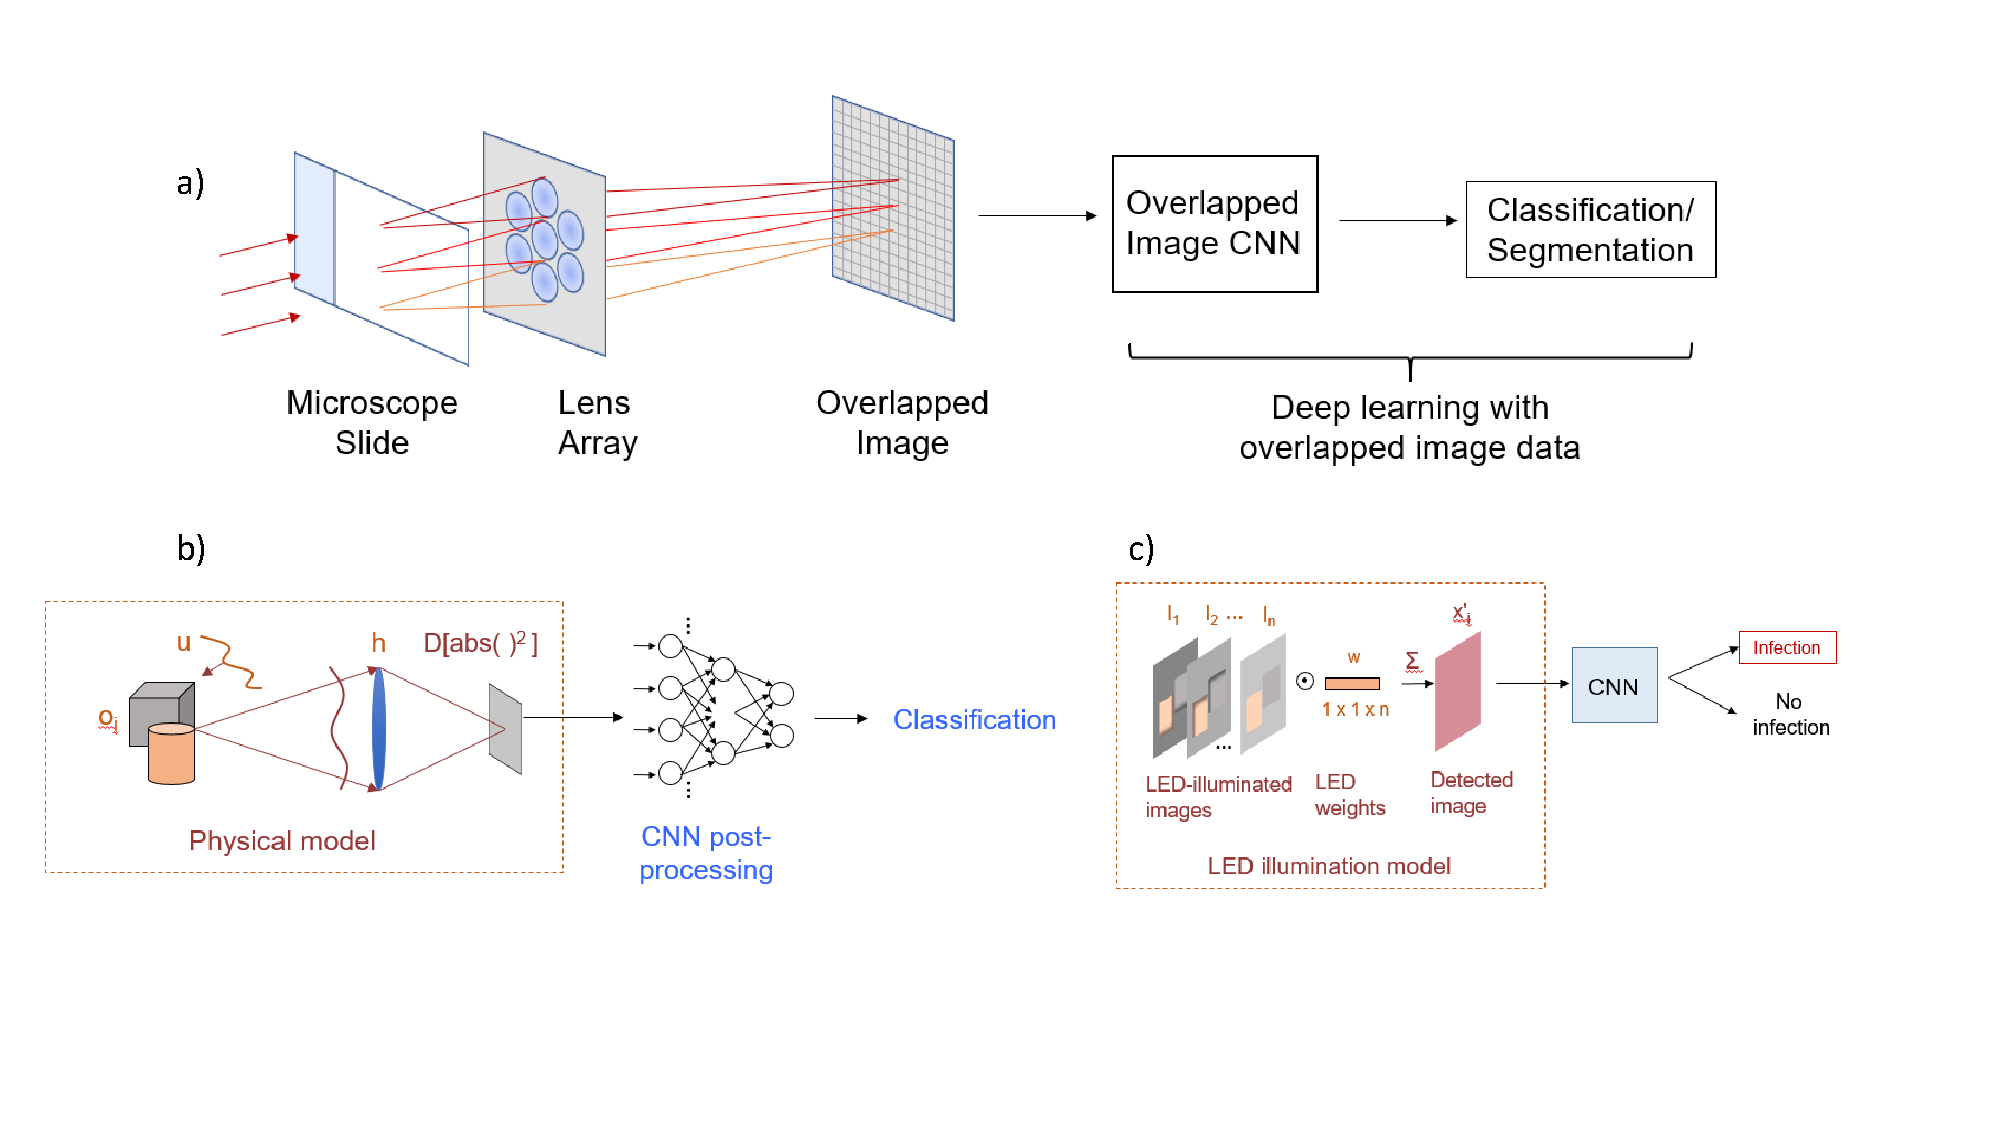
\includegraphics[width=\linewidth]{590L2.pdf}
\caption{(a) An array of small lenses magnify different regions of a sample of interest onto a single image sensor to form an overlapped image. A deep neural network, trained to classify overlapped image data, then classifies different sample regions into classes of interest. (b) Standard imaging setup followed by a digital CNN, (c) Proposed network with the added physical layer used in experiments. Each image, taken under unique LED illumination, is weighted and summed to form the final detected image that then enters the CNN LED weights learned from the physical layer specify the optimal illumination design for our classification microscope.}
\label{simsetup}
\end{figure}

%%%%%%%%%%%%

We also attempt to optimize the hardware of our new microscope design. Our specific goal in this work is to optimize how we illuminate a sample to obtain better performance when we use overlapped imaging for classification of malaria parasite via a supervised machine learning algorithm. We demonstrate that this joint hardware-software optimization process works - it is possible to achieve a significant improvement in cell nuclei segmentation accuracy by also optimizing how the cells are illuminated from a simple and inexpensive matrix of LEDs.

\section{Related work}


There are several existing camera systems that have been designed to detect overlapping images~\cite{Marcia08,Treeaporn10, Horisaki10,Shepard15}. These prior designs are large-scale cameras focused at infinity, as opposed to microscopic imagers with short working distances. There are a number of different strategies to overlap angularly varying FOVs of objects at infinity, as discussed in Ref.~\cite{Shepard15}. However, these are not directly applicable to our goal in the microscope, which is to capture  spatially varying FOVs of a nearby sample on a slide. In addition, the computational goal of the above prior work is to separate out one overlapped image into a set of mutually non-overlapping sub-images, which can then be stitched together into a final composite image. This goal is distinct from our goal here, which is simply to output a classification score from all overlapped regions to indicate the presence or absence of certain features of interest.

In recent years, convolutional neural networks have become commonplace for both medical and natural image classification~\cite{geert}.However, most studies in this area do not attempt to use deep learning to optimize the image acquisition process. While an early work in 1993 used simple neural networks to effectively design components of optical systems \cite{macd}, the first work to the best of our knowledge to examine this question in the context of CNNs was by Chakrabarti \cite{chakrabarti}, who presented an optimal pixel level color-filter layout for color image reconstruction. Subsequent works have considered how the performance of the CNN relates to the underlying optical system \cite{dirty pixels,recon}. However, few of these works have proposed the use of CNNs to optimize the image capturing process itself.

Such an approach was considered by Horstmeyer et al \cite{Horstmeyer17}, who suggested the use of a "physical layer" in a CNN for detection of the malaria parasite. Subsequent work has designed custom optical elements to assist with automated classification~\cite{gordon}, and used machine learning to inform new types of illumination for improved phase contrast imaging \cite{waller,rainer} or superior resolution \cite{ganapati,zheng}. The goal of these works was not to improve the accuracy of an automated task, such as classification or image segmentation, as considered in this work.

\section{Methods}

\subsection{Principle of overlapped imaging}

The general principle of overlapped image classification is shown in Fig.~\ref{simsetup}(a). Instead of relying on a single objective lens, which is limited to a small FOV of just a few square millimeters and cannot be easily improved, our goal here is to use a set of simpler sub-lenses to cover a larger total FOV. Each sub-lens images a unique FOV onto a common image sensor.  With $n$ sub-lenses, our approach can in principle capture light from an $n$ times larger FOV as compared with a standard microscope. While the individual sub-images overlap and thus reduce image contrast, this approach may still be quite useful for tasks where one is searching for a small number of features across a relatively uniform background. The search for the malaria parasite during microscopic diagnosis offers one good example for this type of task, since the parasite can exist just a few times over a square centimeter area in blood smears from infected patients. 

\begin{figure}
\centering
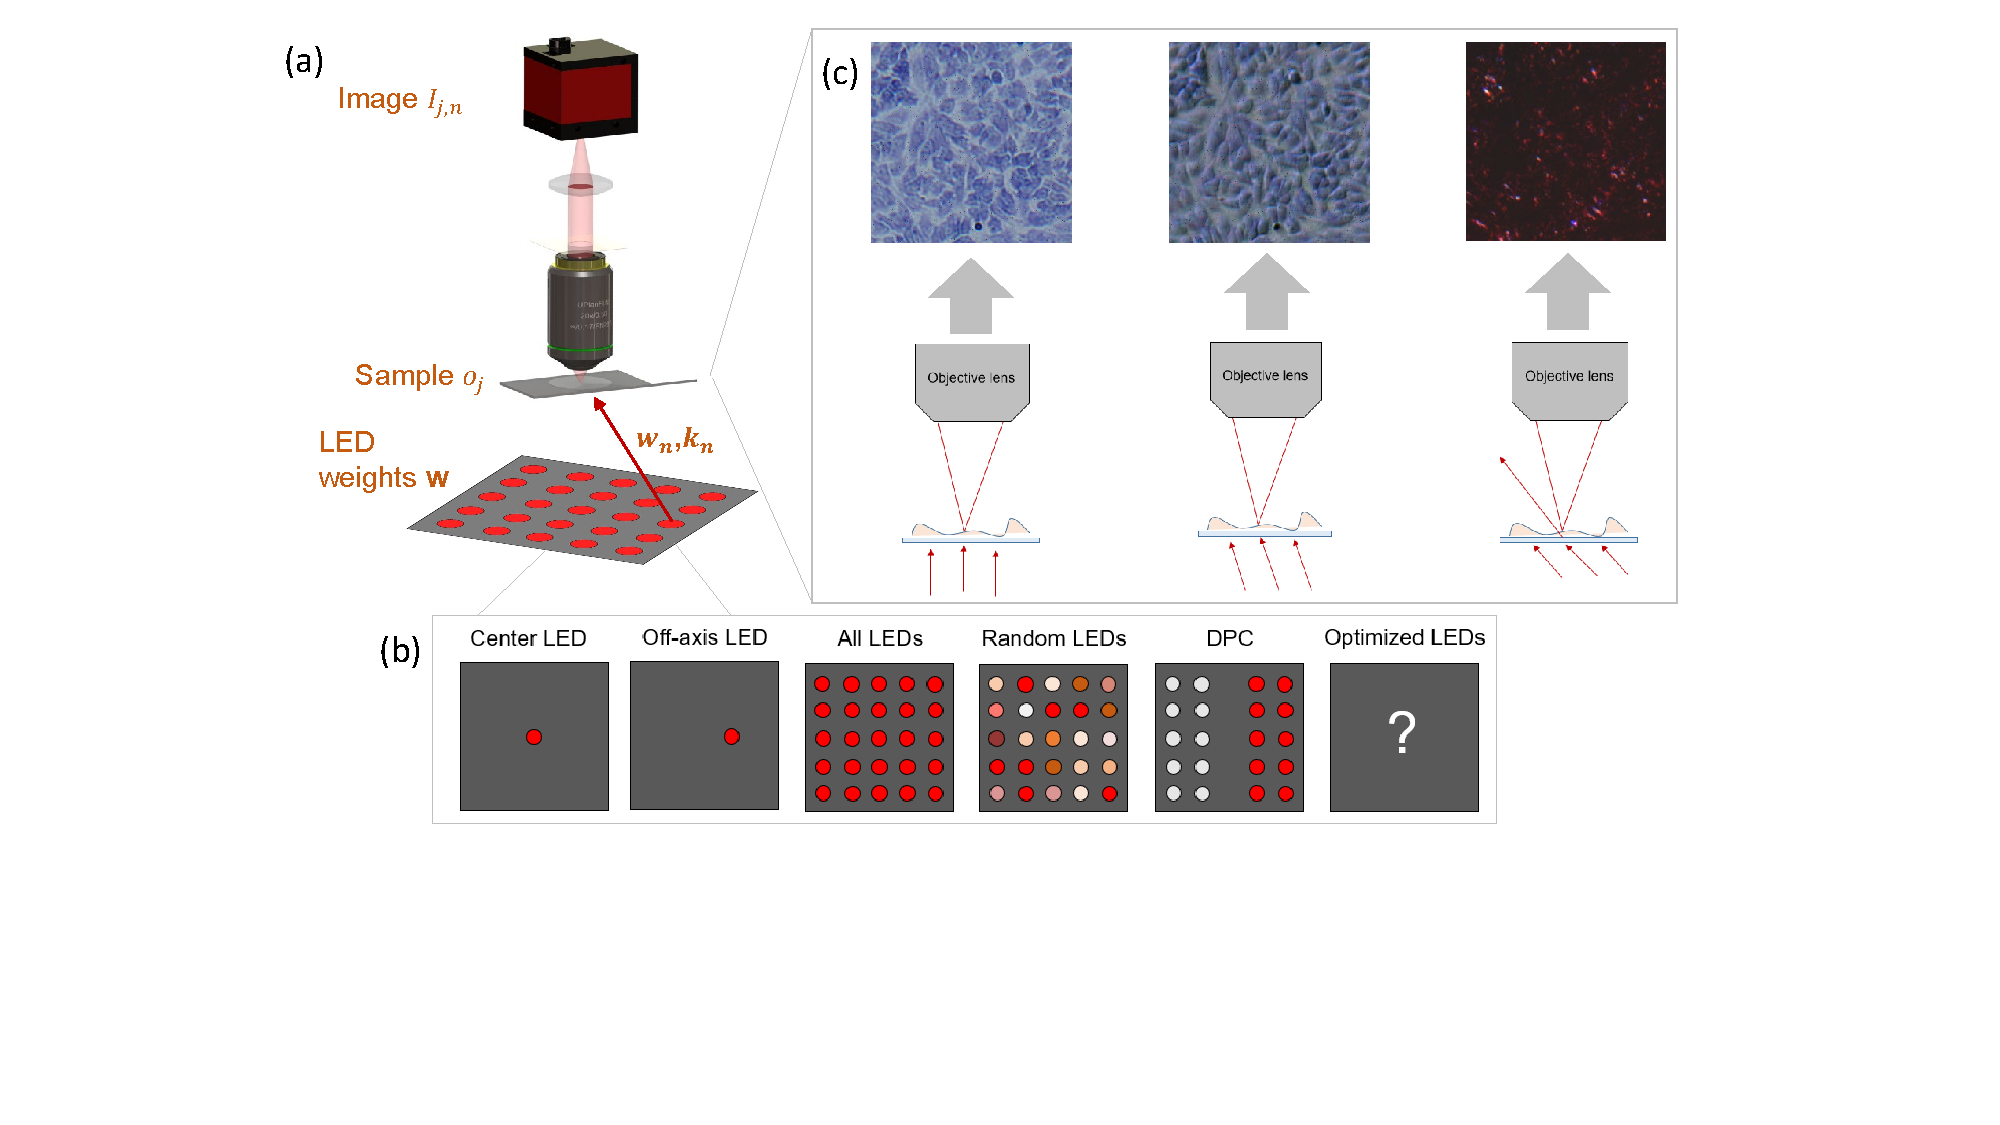
\includegraphics[height=2.25in]{590L4.pdf}
\caption{(a) Transmission microscope imaging configuration, (b) Various illumination patterns used, (c) Effect of the illumination angle on the captured image. From L-R: on-axis illumination, angled illumination to highlight structure due to phase-induced shadows, illumination angle beyond the maximum permissible angle of the lens which produces a dark-field image, highlighting the phase 'bumps'. Contrast of the Dark-field image is digitally enhanced for better viewing.}
\label{led pat}
\end{figure}

In a typical experiment, we illuminate each microscope slide with a single LED placed beneath the sample plane and capture a single image. Our goal is to then classify the presence or absence of the {\it Plasmodium Falciparum} parasite within different areas of this single image that contains overlapping FOVs. Light microscope-based identification of the malaria parasite within a stained blood smear is a common method of diagnosis, especially in resource-limited settings. However, the presence of the parasite is extremely sparse - typically appearing within one out of 100 FOVs of a high-resolution objective lens~\cite{Das15}. By overlapping multiple areas into one snapshot, we hope to increase the probability of detecting a parasite and thus the efficiency of detection while still offering a high classification accuracy. Our slides contain thick blood smears, in which the cell bodies have been lysed to create a large non-uniform background. This is a commonly used preparation for diagnosis~\cite{Das15}. This non-uniform background makes is quite challenging to determine the presence of infection even in a non-overlapped image, but it increases the density of the parasite along the slide surface for a more efficient diagnosis. Our goal here is to further increase this efficiency by a factor of $n$ by capturing data from an $n$ times larger area in one snapshot.

\subsection{Principle of physical layer}

In a standard microscope, light propagates from an illumination source to the object(s) of interest, interacts with the object physically, propagates through a light collection element and then reaches an image sensor. The sensor discretizes the incident radiation to generate a digital image. This process is illustrated in Fig \ref{simsetup}(b). Normally, work within the machine learning community relies on large pre-recorded image sets from standard microscopes, and does not consider the above physical parameters that can significantly alter the appearance of each captured microscope image.

Here, we propose to model this physical image formation process as a set of learnable weights within the early layers of our neural network, which are typically referred to as "physical layers". Each physical layer weight corresponds to an aspect of data collection hardware. In this work, our physical layer models microscope illumination, and we append it to the front of the CNN to improve classification. After the network is trained, the optimized weights within the physical layers (in this case, the angular and spectral distribution of sample illumination) inform us of a better optical design for the task at hand.

In our experimental setup, we use a discrete set of 123 LED illuminators to define our sample illumination, as represented in Fig \ref{led pat}(a). Illumination from a wide variety of angles provides diverse spectral and thickness information about an object that is not available under normal illumination conditions. For example, as shown in Fig \ref{led pat}(c), if plane wave illumination is incident upon an object from a large angle, we can see phase-induced shadows at the edges of sample sub-structures (here, cell bodies). Similarly, if the angle of incident radiation is increased beyond the maximum acceptance angle of the microscope lens, we will capture dark-field images that highlight 'bumps' at locations of sample thickness variation. In our approach, we aim to use a machine learning model to identify the most useful pieces of information for the task at hand.

Formally, The detected image under illumination from a particular LED pattern is:
\begin{equation}
I_j^\prime = \sum_{\lambda} \sum_{n=1}^N w_n(\lambda)I_{j,n}.
\label{eq:phys_layer}
\end{equation}
where each LED has a brightness $w_n(\lambda)$, is equal to the weighted sum of images captured by turning on each LED individually and we denote the image of the $j$th sample formed when it is illuminated by the $n$th LED at a fixed brightness and wavelength as $I_{j,n}(\lambda)$ Our goal is to train an image classification model that also outputs an ideal set of weights $w_n(\lambda)$. To do so, we need a set of $N$ uniquely illuminated images $\{I_{j,n}\}_{n=1}^N$ for each object of interest $o_j$ during network training. After training, the optimized LED weight vector $\mathbf{w}$ tells us how to illuminate all of the LEDs \emph{simultaneously} to take a single optimally illuminated picture. This picture will enter the trained CNN for better classification. An illustration of this process is shown in Figure \ref{simsetup}(c) In this way, we can easily experimentally realise the optimal LED illumination model from Fig \ref{fig:led pat}(b).

\section{Simulation}

\subsection{Digital Overlapping}
To create the training set for overlapped imaging, we can first capture many non-overlapping images from a standard microscope setup and then digitally generate overlapped images by averaging different combinations of $n$ non-overlapped images. We can do this process with two different optical illumination schemes. First to set a baseline, we will only light up the center LED and record the images to average later. Then to investigate optimized illumination, we can illuminate the using a programmable LED array and record a set of uniquely illuminated images for each sample. For overlapping multiple sets, we would then average images from each LED and create an output set with the same number of images as one of the original stacks.

\begin{figure}
\centering
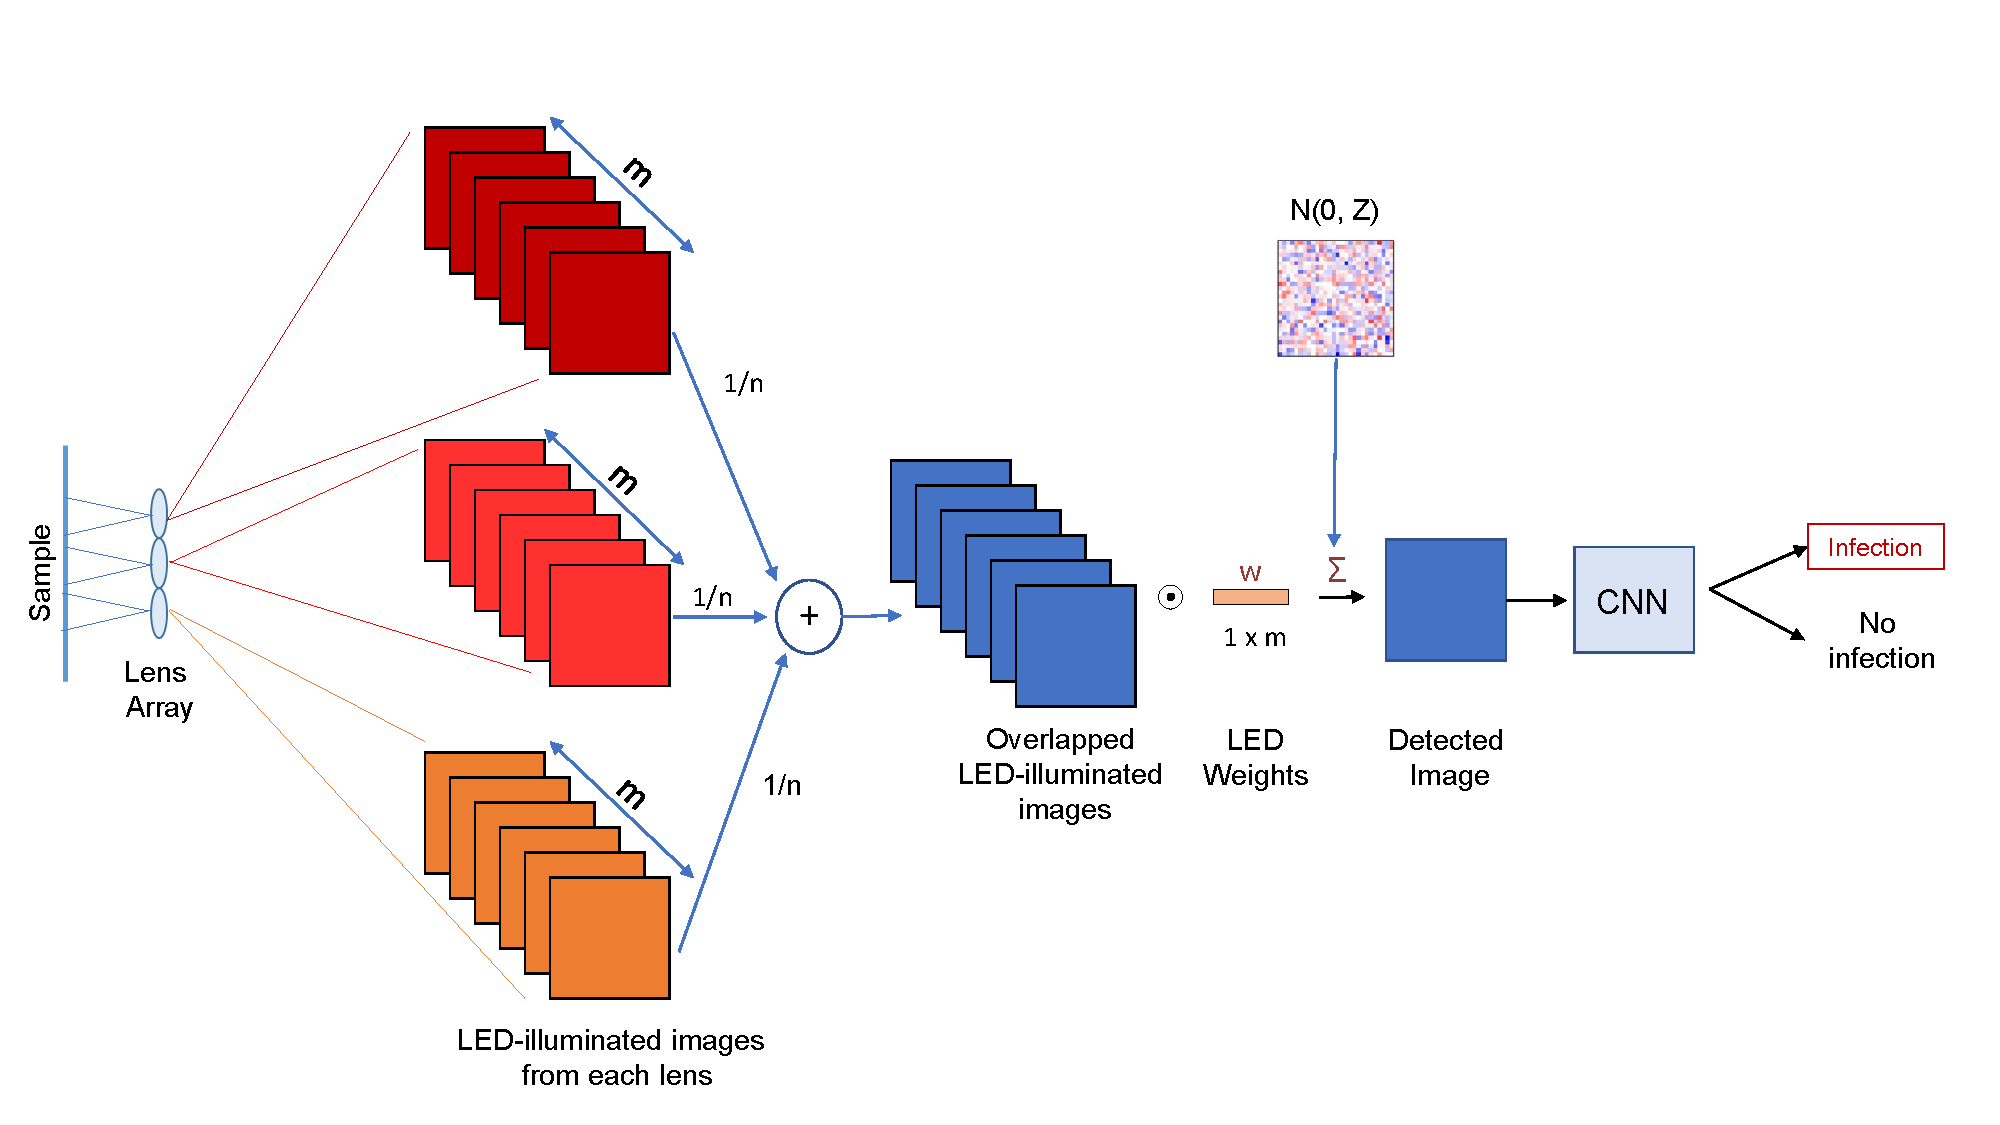
\includegraphics[width=\linewidth]{590L1.pdf}
\caption{Illustration of the digital overlapping process alongwith the illumination optimization}
\label{digitaloverlap}
\end{figure}

We first captured standard microscope images of blood smear slides containing the {\it P. Falciparum} parasite using an upright microscope with similar lens specifications (10X, NA=0.28, Mitutoyo), sensor specifications (3.45 $\mu$m pixels, Sony IMX, monochrome) and illumination (single white LED placed 10 cm beneath sample). We then had an expert manually identify the malaria parasites in the standard slide images, based on which we isolated 28$\times$28-pixel patches of both malaria-infected and non-malaria-infected cells.

Then, we "digitally overlapped" these 28$\times$28-pixel images, by simply adding together $n$ different labeled examples from different locations along the FOV (see Fig.~\ref{digitaloverlap}), and discretizing/normalizing appropriately. These digitally averaged images form our examples for network training. In case of training for optimized illumination, we also performed a weighted addition of images from all the unique LEDs, after overlapping, to generate the image given to the neural network. Optimal weights for this step are to be learned by the network.

To generate $n$-overlapped images, as outlined in Fig. \ref{digitaloverlap}, we took the mean of the $n$ images, added random zero-mean Gaussian noise (the variance is described in the next paragraph), and discretized the result into 8 bits. For malaria-positive samples, exactly 1 of the $n$ images contained a malaria parasite; for malaria-negative samples, none of the $n$ images contained parasites. Examples are shown in Fig. \ref{digitaloverlap}(b). Our raw, un-overlapped dataset consisted of 705 malaria-infected image patches and 692 non-infected image patches, and the many linear combinations of these examples lead to a sizable overlapped image training set. Each of the patches was imaged using 41 unique LEDs and using three colors: red, green and blue. So we have 123 images per datapoint.

Because we digitally synthesized the $n$-overlapped images, in addition to addressing the dynamic range we must also correct for the amount of noise in the final image. In particular, after averaging $n$ individually captured images, the resulting overlapped image has an artifactual $\sqrt{n}$ improvement in SNR. Thus, to artificially inflate the amount of noise to accurately simulate a physically overlapped image, we added a normally distributed random variable $Z[i,j] \sim N(\mu=0,\sigma^2=X_{avg}[i,j](1-1/n)2^{n_{bit}}/v)$ pixel-wise to the averaged image $X_{avg}$, where $n_{bit}=8$ is the bit depth of the camera and $v$ is full well depth of the camera pixel. We prove in the Appendix that $X_{avg}+Z$ has the correct mean and variance in the shot noise limit.

\subsection{CNN design for overlapped imaging}

The images input for training are single-channel (monochromatic) and contain 28$\times$28 pixels, which are then processed by four convolutional layers with 3$\times$3 filters, with 32, 32, 64, and 64 filters respectively, followed by one fully connected layer (3136 input units, 1024 output units) before finally being processed through a softmax output, from which the cross-entropy loss is computed. The second and fourth convolutional layers are strided by 2 to reduce the input image size. Layer normalization~\cite{layernorm} is used after the second and fourth convolutional layers as well as after the fully connected layer. All activations are ReLU. We trained the network in TensorFlow using the Adam optimizer with a learning rate of 1e-4 and a batch size of 32 for 250 iterations for each $n$ for baseline measurements. For optimized illumination scheme, we need to train for longer since there is an additional physical layer added to the network. It was trained for 500 iterations for this scheme. Training and testing examples were generated on the fly for both the cases.

\section{Results}

Fig. \ref{overlapgraph}(a) plots the results of our digital overlap classification experiment. Two curves: for center illumination and optimized illumination are shown. 

\begin{figure}
\centering
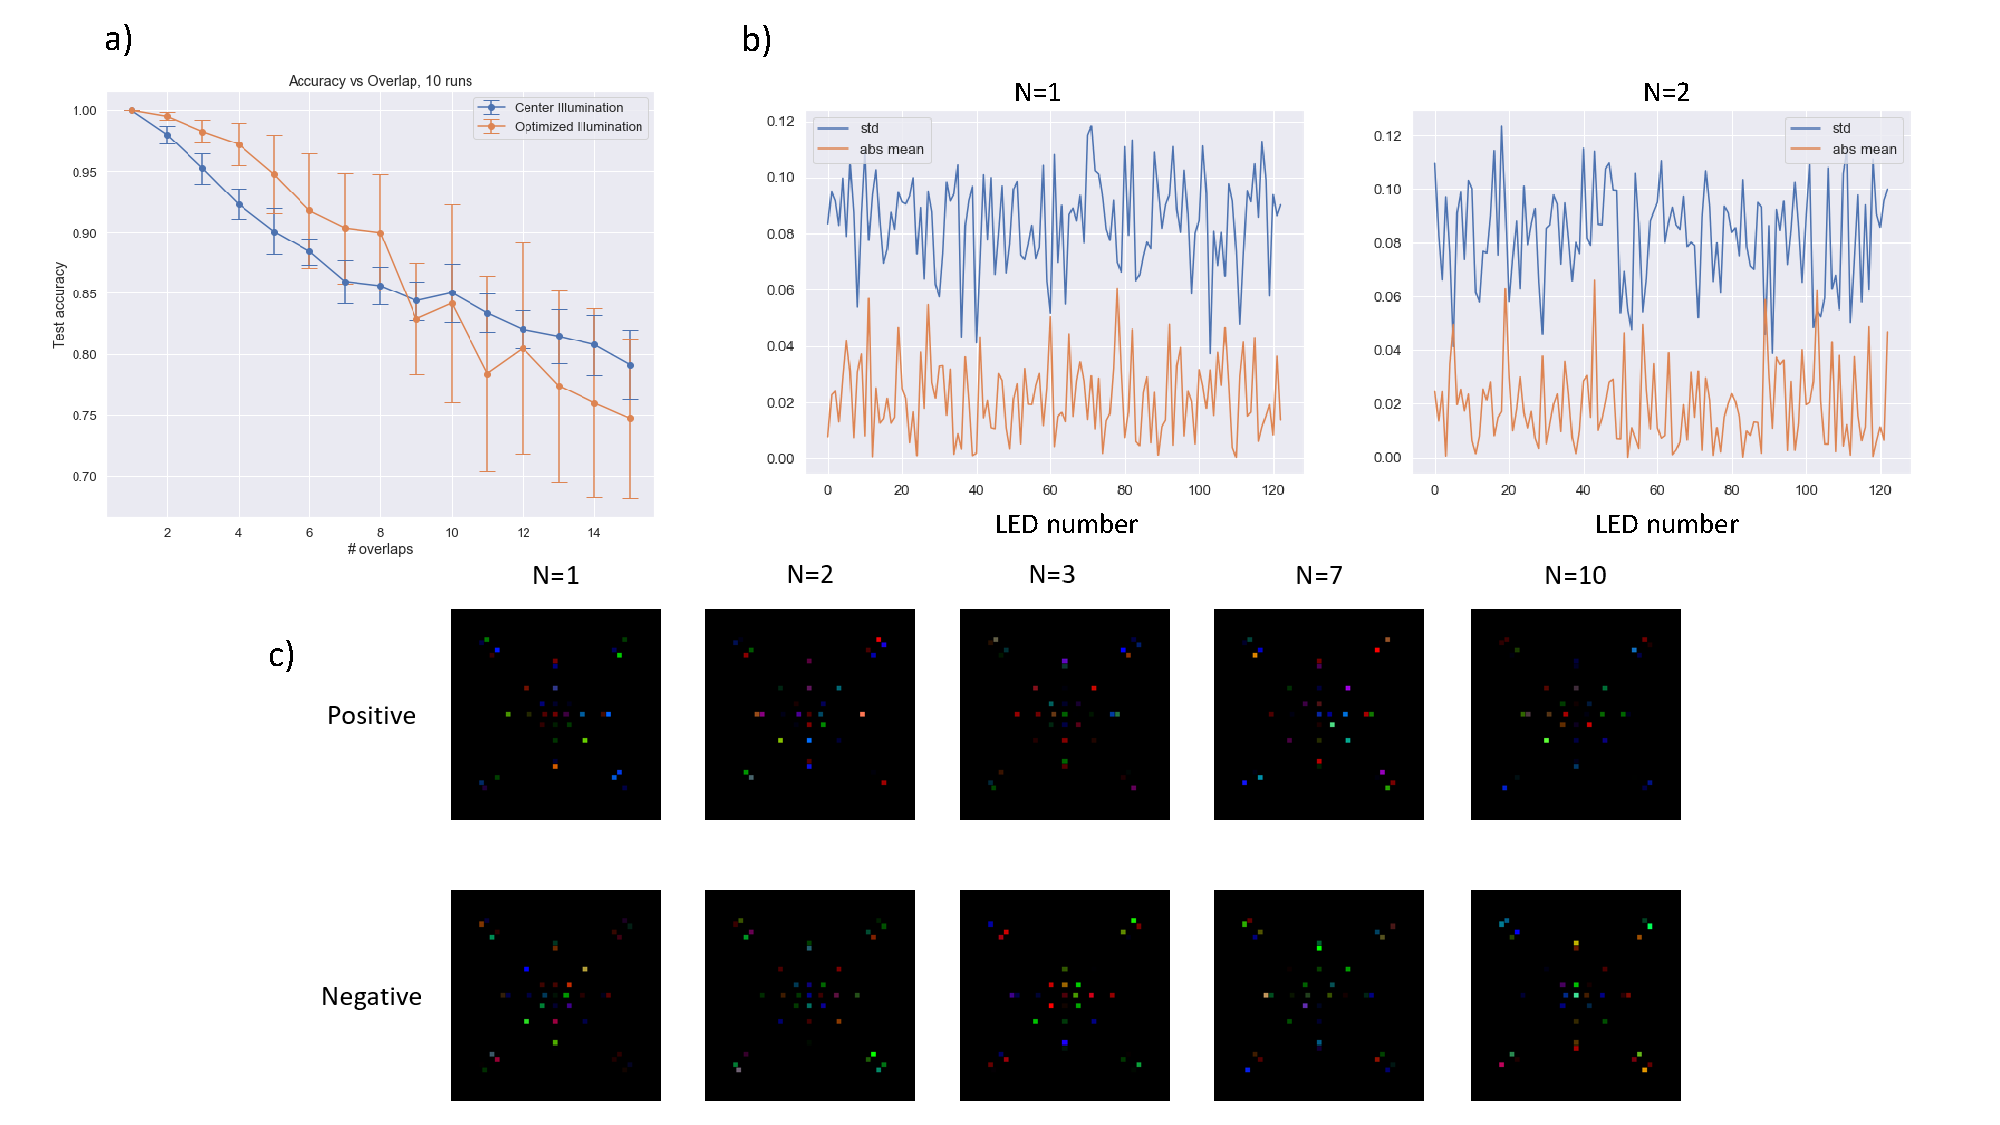
\includegraphics[width=\linewidth]{590L3.pdf}
\caption{(a) Classification accuracy versus number of overlapped images $n$. Each plot point is an average of 10 independent trials with varied input training/testing datasets and using random weight initialization. (b) plot of variation of LED weights obtained after training for $n=1$ and 2. (c) Mean optimized patterns obtained for some of the values of $n$}
\label{overlapgraph}
\end{figure}

For center illumination, our CNN classifies the malaria parasite with approximately 98\% accuracy on standard images with no overlap ($n=1$). This classification accuracy decreases a function of image overlap parameter. At $n=4$ overlapped images, the accuracy of our classifier still remains above 90\%. To a human observer, the distinction between malaria-positive and negative examples becomes relatively unclear at 3 or 4 overlapped images. Somewhat surprisingly, our neural network maintains over 80\% accuracy until an overlap parameter of approximately $n=10$. For overlap parameters greater than 10, the classification accuracy variance begins to increase. We performed experiments with up to $n=15$ overlaps using this scheme, and neural network accuracies remained in excess of 70\%, which indicates that there may be some overfitting in our experiments. However, the general trend of Fig. \ref{overlapgraph}(a) follows our expectations and we can conclude that overlapped imaging remains an effective strategy for high-throughput classification for lower values of image overlap, especially given a certain amount of tolerance to classification accuracy. With optimized illumination scheme, the accuracy of the network is improved upto $n=8$ and then we see a surprising and sudden drop in performance. The variance in results is also quite high. The learned weights are shown in Fig \ref{overlapgraph}(c) but, these also show very high variance as demonstrated in the representative plots of Fig \ref{overlapgraph}(b). A further investigation in the cause for the high variance is required and presents a clear direction for future work.

In summary we have demonstrated a new optical system that can capture images of multiple unique fields-of-view overlapped on a common detector, which may offer a significant potential speed-up for automated image classification. We have also shown that optimizing physical parameters of the optical system simultaneously with the neural network can improve performance even for the difficult task of classifying overlapped images.


%%%%%%%%%%%%%%%%%%%%%%%%%%%%%%%%%%%%%%%
%Bibliography

\begin{thebibliography}{99}

\bibitem{Zheng14} G. Zheng, X. Ou, R. Horstmeyer, J. Chung, C. Yang, ``Fourier ptychographic microscopy: A gigapixel superscope for biomedicine," Optics and Photonics News {\bf 25}(4), 26--33 (2014).

\bibitem{Lohmann} A. W. Lohmann, ``Scaling laws for lens systems," Applied Optics {\bf 28}(23), 4996-4998 (1989).

\bibitem{Brady12} D. J. Brady et al., ``Multiscale gigapixel photography," Nature {\bf 486}, 286--289 (2012).

\bibitem{Zheng13} G. Zheng, R. Horstmeyer and C. Yang, ``Wide-field, high-resolution Fourier ptychographic microscopy," Nature Photonics {\bf 7}, 739--745 (2013).

\bibitem{Yuan17} X. Yuan et al., ``Multiscale gigapixel video: A cross resolution image matching and warping approach," IEEE ICCP (2017).

\bibitem{Liu17} Y. Liu et al., ``Detecting cancer metastases on gigapixel pathology images," ArXiv:1703.02442v2 (2017).

\bibitem{Angelova15} A. Angelova, A. Krizhevsky, and V. Vanhoucke, ``Pedestrian detection with a large-field-of-view
deep network," International Conference on Robotics and Automation ICRA (2015).

\bibitem{Horstmeyer17} R. Horstmeyer, R. Y. Chen, B. Kappes and B. Judkewitz, ``Convolutional neural networks that teach
microscopes how to image," arXiv:1709.07223 (2017).

\bibitem{Marcia08} R. F. Marcia et al., ``Superimposed video disambiguation for increased field of view," Opt. Express {\bf 16},  16352--16363 (2008).

\bibitem{Treeaporn10} V. Treeaporn, A. Ashok and M. A. Niefeld, ``Increased field of view through optical multiplexing," Opt. Express {\bf 18}, 22432--22445 (2010).

\bibitem{Horisaki10} R. Horisaki and J. Tanida, ``Multi-channel data acquisition using multiplexed imaging with spatial encoding," Opt. Express {\bf 18}, 23041--23053 (2010).

\bibitem{Shepard15} R. Hamilton Shepard, Y. Rachlin, V. Shah and T. Shih, ``Design architectures for optically multiplexed images," Opt. Express {\bf 23}, 31419--31436 (2015).

\bibitem{geert}
Litjens G., et al.: A Survey on Deep Learning in Medical Image Analysis. Med Image Anal. \textbf{42}, 60--88 (2017).

\bibitem{macd}
J. Macdonald et al.: Optimization of a Lens Design Using a Neural
Network. In Proc. SPIE 1965, Applications of Artificial Neural Networks IV, 431 (1993).

\bibitem{chakrabarti}
A. Chakrabarti.: Learning Sensor Multiplexing Design through Back-propagation. In Adv.
Neural Inf. Proc. Sys. (NIPS) 2016, 3081--3089 (2016).

\bibitem{dirty pixels}
Diamond S., et al.: Dirty pixels: Optimizing image
classification architectures for raw sensor data. arXiv:1701.06487 (2017).

\bibitem{recon}
Kulkarni K., et al.: ReconNet: Non-Iterative Reconstruction of Images from Compressively Sensed Random Measurements. arXiv:1601.06892 (2016).

\bibitem{gordon}
Sitzmann V., et al.: End-to-end Optimization of Optics and Image Processing for Achromatic Extended Depth of Field and Super-resolution Imaging. In ACM SIGGRAPH (2018).

\bibitem{waller}
Kellman M., et al.: Physics-based Learned Design: Optimized Coded-Illumination for Quantitative Phase Imaging. arXiv:1808.03571 (2018).

\bibitem{rainer}
Diederich B., et al.: Using machine-learning to optimize phase contrast in a low-cost cellphone microscope. PLOS ONE \textbf{13}(3): e0192937 (2018).

\bibitem{ganapati}
Y.F. Cheng, et al.: Illumination pattern design with deep learning for single-shot Fourier ptychographic microscopy. Opt. Express \textbf{27}, 644--656 (2019)

\bibitem{zheng} S. Jiang et al., Solving Fourier ptychographic imaging problems via neural network modeling and TensorFlow, \textbf{9} Biomed. Opt. Express (2018).

\bibitem{Das15} D. K. Das, R. Mukherjee and C. Chakraborty, ``Computational microscopic imaging for malaria parasite detection: a systematic review," J. Microscopy {\bf 260}, 1--19 (2015).

 \end{thebibliography}
 

\end{document}



%%%%%%%%%%%%%%%%%%%%%%
%%Experimental results table, thin smear, with center LED
%\begin{table}[b]
%  \caption{DP-CNN classification of {\it P. falciparum} infection, thin smear, with center LED}
%  \label{sample-table}
%  \centering
%  \begin{tabular}{lllllllll}
%    \toprule
%   \multicolumn{2}{c}{ }     & \multicolumn{7}{c}{Illumination Type \& Classification Score}               \\
%    \cmidrule{3-9}
%    Data & Value & Center & Off-axis & DPC & All & Random & PC Ring & Optim.   \\
%    \midrule
%    %Red-only & Average & 0.829 & 0.713 & 0.708 & 0.710 & 0.724 & 0.845 & 0.862 \\
%     %& Majority & 0.849 & 0.722 & 0.723 & 0.722 & 0.759 & 0.854 & {\bf 0.894} \\
%     %& STD & 0.013 & 0.015 & 0.011 & 0.012 & 0.046 & 0.011 & 0.018  \\
%    \midrule
%    %This was the second run with the PC Ring data, I messed up the first run
%     Red-only & Average & 0.839 & 0.772 & 0.708 & 0.781 & 0.762 & 0.881 & 0.890 \\
%     & Majority & 0.845 & 0.796 & 0.715 & 0.797 & 0.797 & 0.891 & {\bf 0.906} \\
%     & STD & 0.017 & 0.016 & 0.011 & 0.018 & 0.045 & 0.011 & 0.011  \\
%    \midrule
%    Green-only & Average & 0.873 & 0.736 & 0.717 & 0.727 & 0.772 & 0.900 & 0.897 \\
%     & Majority & 0.885 & 0.739 & 0.721 & 0.755 & 0.834 & 0.911 & {\bf 0.915}  \\
%     & STD & 0.022 & 0.010 & 0.017 & 0.012 & 0.046 & 0.011 & 0.016 \\
%    \midrule
%    Blue-only & Average & 0.869 & 0.745 & 0.792 & 0.753 & 0.813 & 0.881 & 0.887 \\
%     & Majority & 0.875 & 0.761 & 0.816 & 0.766 & 0.875 & 0.895 & {\bf 0.922}  \\
%     & STD & 0.012 & 0.015 & 0.006 & 0.014 & 0.032 & 0.014 & 0.017 \\
%     \midrule
%     RGB, cent init & Average & 0.917 & 0.779 & 0.750 & 0.727 & 0.785 & 0.879 & 0.928 \\
%     & Majority & 0.935 & 0.799 & 0.770 & 0.744 & 0.833 & 0.911 &{\bf 0.946}  \\
%     & STD & 0.005 & 0.006 & 0.009 & 0.022 & 0.028 & 0.011 & 0.007 \\
%    \bottomrule
%  \end{tabular}
%\end{table}



%%%%%%%%%%%%%%%%%%%%%
%Experimental results table, thin smear, with center LED
%NOTE 11/7/18: This table is before adding the PC-ring results, in which case I took both the 
%PC Ring score from the new run, and the optimized case score from the new one
% The rest of the scores, including the center score, did not change at all really
%\begin{table}[b]
%  \caption{DP-CNN classification of {\it P. falciparum} infection, thin smear, with center LED}
%  \label{sample-table}
%  \centering
%  \begin{tabular}{llllllll}
%    \toprule
%   \multicolumn{2}{c}{ }     & \multicolumn{6}{c}{Illumination Type \& Classification Score}               \\
%    \cmidrule{3-8}
%    Data & Value & Center & Off-axis & DPC & All & Random & Optim.   \\
%    \midrule
%    Red-only & Average & 0.829 & 0.713 & 0.708 & 0.710 & 0.724 & {\bf 0.852} \\
%     & Majority & 0.849 & 0.722 & 0.723 & 0.722 & 0.759 & {\bf 0.868} \\
%     & STD & 0.013 & 0.015 & 0.011 & 0.012 & 0.046 & 0.016  \\
%    \midrule
%    Green-only & Average & 0.873 & 0.736 & 0.717 & 0.727 & 0.772 & {\bf 0.883} \\
%     & Majority & 0.885 & 0.739 & 0.721 & 0.755 & 0.834 & {\bf 0.900}  \\
%     & STD & 0.022 & 0.010 & 0.017 & 0.012 & 0.046 & 0.016 \\
%    \midrule
%    Blue-only & Average & 0.869 & 0.745 & 0.792 & 0.753 & 0.813 & {\bf 0.883} \\
%     & Majority & 0.875 & 0.761 & 0.816 & 0.766 & 0.875 & {\bf 0.910}  \\
%     & STD & 0.012 & 0.015 & 0.006 & 0.014 & 0.032 & 0.023 \\
%%    \midrule
%%     RGB 3K, rand init & Average & 0.875 & 0.747 & 0.739 & 0.713 & 0.766 & 0.877 \\
%%     & Majority & 0.893 & 0.752 & 0.748 & 0.724 & 0.830 & 0.901  \\
%%     & STD & 0.017 & 0.022 & 0.016 & 0.020 & 0.032 & 0.018 \\
%     \midrule
%     RGB, cent init & Average & 0.918 & 0.779 & 0.750 & 0.727 & 0.785 & {\bf 0.930} \\
%     & Majority & 0.933 & 0.799 & 0.770 & 0.744 & 0.833 & {\bf 0.941}  \\
%     & STD & 0.005 & 0.006 & 0.009 & 0.022 & 0.028 & 0.007 \\
%    \bottomrule
%  \end{tabular}
%\end{table}
